\documentclass{beamer}
\usepackage[utf8]{inputenc}

\usetheme{Madrid}
\usecolortheme{default}
\usepackage{amsmath,amssymb,amsfonts,amsthm}
\usepackage{txfonts}
\usepackage{tkz-euclide}
\usepackage{listings}
\usepackage{adjustbox}
\usepackage{array}
\usepackage{tabularx}
\usepackage{gvv}
\usepackage{lmodern}
\usepackage{circuitikz}
\usepackage{tikz}
\usepackage{graphicx}

\setbeamertemplate{page number in head/foot}[totalframumber]

\title{2.7.25}

\author{EE25BTECH11013 - Bhargav}
\date{August 29, 2025}

\begin{document}

\frame{\titlepage}

\begin{frame}{Question}
Find the area of quadrilateral $ABCD$ whose vertices are $A(-3,-1)$, $B(-2,-4)$, $C(4,-1)$ and $D(3,4)$.
\end{frame}

\begin{frame}{Theoretical Solution}
The area of the quadrilateral can be found by dividing it into 2 triangles, $\triangle ABC$ and $\triangle ACD$, and then summing their areas.
\vfill
The area of a triangle formed by vectors $\vec{u}$ and $\vec{v}$ originating from the same vertex is given by:
\begin{align}
    \text{Area} = \frac{1}{2} | \vec{u} \times \vec{v} |
\end{align}
\vfill
The given vertices are:
\begin{align}
    \vec{A} = \myvec{-3 \\ -1} \quad
    \vec{B} = \myvec{-2 \\ -4} \quad
    \vec{C} = \myvec{4 \\ -1} \quad
    \vec{D} = \myvec{3 \\ 4}
\end{align}
\end{frame}

\begin{frame}{Calculation: Triangle ABC}

\begin{align}
\vec{A}-\vec{B} 
= \myvec{-3+2 \\ -1+4} = \myvec{-1 \\ 3}
\end{align}


\begin{align}
\vec{A} - \vec{C} = \myvec{-3-4 \\ -1+1} = \myvec{-7 \\ 0}
\end{align}



\begin{align}
(\triangle ABC)=\frac{1}{2}\norm{(\vec{A}-\vec{B}) \times (\vec{A}-\vec{C})}
\end{align}

\begin{align}
(\triangle ABC)=\frac{1}{2}\norm{\myvec{-1 \\ 3} \times \myvec{-7 \\ 0}}=\frac{1}{2}\cdot 21=\frac{21}{2}.
\end{align}

\end{frame}

\begin{frame}{Calculation: Triangle ACD}

\begin{align}
\vec{A}-\vec{D}
=\myvec{-3-3 \\ -1-4} = \myvec{-6 \\ -5}  
\end{align}


\begin{align}
(\triangle ACD)=\frac{1}{2}\norm{(\vec{A}-\vec{C}) \times (\vec{A}-\vec{D})}=\frac12\cdot 35=\frac{35}{2}
\end{align}

\end{frame}

\begin{frame}{Final Result}
The total area of the quadrilateral $ABCD$ is the sum of the areas of the two triangles.
\begin{align}
    \text{Area}(ABCD) &= \text{Area}(\triangle ABC) + \text{Area}(\triangle ACD) \\
    &= \frac{21}{2} + \frac{35}{2} \\
    &= \frac{56}{2} \\
    &= 28
\end{align}
\vfill
\textbf{Therefore, the area of the quadrilateral is 28 square units.}
\end{frame}


\begin{frame}[fragile]
    \frametitle{C Code}
    \begin{lstlisting}
#include <stdio.h>
#include <math.h>


double cross2D(double x1, double y1, double x2, double y2) {
    return fabs(x1*y2 - y1*x2);
}


double triangle_area(double ax, double ay, double bx, double by, double cx, double cy) {
    double v1x = bx - ax;
    double v1y = by - ay;
    double v2x = cx - ax;



    \end{lstlisting}
\end{frame}

\begin{frame}[fragile]
    \frametitle{C Code}
    \begin{lstlisting}
    double v2y = cy - ay;
    return 0.5 * cross2D(v1x, v1y, v2x, v2y);
}


double quad_area(double ax, double ay, double bx, double by, double cx, double cy, double dx, double dy) {
    double area1 = triangle_area(ax, ay, bx, by, cx, cy);
    double area2 = triangle_area(ax, ay, cx, cy, dx, dy);
    return area1 + area2;
}

    \end{lstlisting}
\end{frame}

\begin{frame}[fragile]
    \frametitle{Python + C Code}
    \begin{lstlisting}
import ctypes
import numpy as np
import matplotlib.pyplot as plt


lib = ctypes.CDLL("./libquad.so")


lib.triangle_area.argtypes = [ctypes.c_double, ctypes.c_double,
                              ctypes.c_double, ctypes.c_double,
                              ctypes.c_double, ctypes.c_double]
lib.triangle_area.restype = ctypes.c_double


    \end{lstlisting}
\end{frame}

\begin{frame}[fragile]
    \frametitle{Python + C Code}
    \begin{lstlisting}
lib.quad_area.argtypes = [ctypes.c_double, ctypes.c_double,
                          ctypes.c_double, ctypes.c_double,
                          ctypes.c_double, ctypes.c_double,
                          ctypes.c_double, ctypes.c_double]
lib.quad_area.restype = ctypes.c_double

# Vertices of quadrilateral
A = (-3.0, -1.0)
B = (-2.0, -4.0)
C = (4.0, -1.0)
D = (3.0, 4.0)


area = lib.quad_area(A[0], A[1], B[0], B[1], C[0], C[1], D[0], D[1])
print("Area of Quadrilateral ABCD =", area)

    \end{lstlisting}
\end{frame}

\begin{frame}[fragile]
    \frametitle{Python + C Code}
    \begin{lstlisting}
points = np.array([A, B, C, D, A])  
plt.plot(points[:,0], points[:,1], 'b-o')
plt.fill(points[:,0], points[:,1], color='skyblue', alpha=0.5)
plt.text(A[0], A[1], "A")
plt.text(B[0], B[1], "B")
plt.text(C[0], C[1], "C")
plt.text(D[0], D[1], "D")

plt.title(f"Quadrilateral ABCD (Area = {area:.2f})")
plt.xlabel("x")
plt.ylabel("y")
plt.grid(True)
plt.axis("equal")
plt.savefigs("/Users/bhargavkrish/Documents/ee1030-2025/ee25btech11013/matgeo/2.7.25/figs/Figure_1.png")
plt.show()

    \end{lstlisting}
\end{frame}



\begin{frame}[fragile]
    \frametitle{Python Code}
    \begin{lstlisting}
import numpy as np
import matplotlib.pyplot as plt


def triangle_area(A, B, C):
    v1 = np.array(B) - np.array(A)
    v2 = np.array(C) - np.array(A)
    return 0.5 * abs(np.cross(v1, v2))


def quad_area(A, B, C, D):
    return triangle_area(A, B, C) + triangle_area(A, C, D)




    \end{lstlisting}
\end{frame}

\begin{frame}[fragile]
    \frametitle{Python Code}
    \begin{lstlisting}

A = (-3, -1)
B = (-2, -4)
C = (4, -1)
D = (3, 4)

area = quad_area(A, B, C, D)
print("Area of Quadrilateral ABCD =", area)

points = np.array([A, B, C, D, A])  
plt.plot(points[:,0], points[:,1], 'b-o')
plt.fill(points[:,0], points[:,1], color='lightgreen', alpha=0.5)



    \end{lstlisting}
\end{frame}

\begin{frame}[fragile]
    \frametitle{Python Code}
    \begin{lstlisting}

for point, label in zip([A, B, C, D], ["A", "B", "C", "D"]):
    plt.text(point[0], point[1], label, fontsize=12, ha='right')

plt.title(f"Quadrilateral ABCD (Area = {area:.2f})")
plt.xlabel("x")
plt.ylabel("y")
plt.grid(True)
plt.axis("equal")
plt.savefig("/Users/bhargavkrish/Documents/ee1030-2025/ee25btech11013/matgeo/2.7.25/figs/Figure_1.png")
plt.show()


    \end{lstlisting}
\end{frame}

\begin{frame}{Plot}
    \centering
    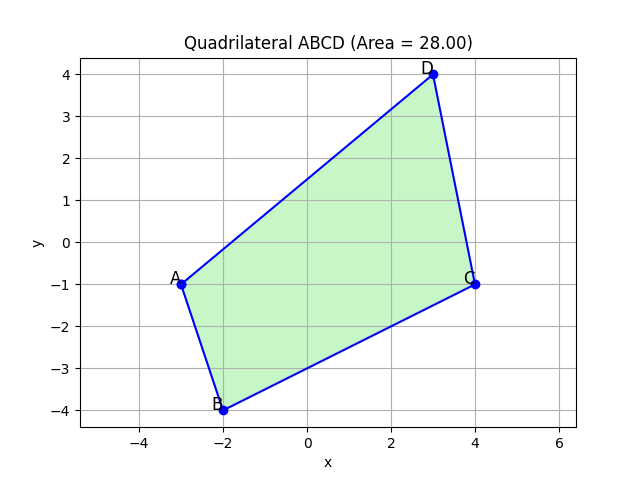
\includegraphics[width=\columnwidth, height=0.8\textheight, keepaspectratio]{figs/Figure_1.png}   
\end{frame}

\end{document}